\documentclass[a4paper, 10pt]{article}
\usepackage{pgf}
\usepackage{eurosym}
\usepackage{graphicx}
\usepackage{wasysym}
\usepackage{hyperref}
\usepackage{listings}
\usepackage{pxfonts}
\usepackage{verbatim}
\usepackage{color}
\usepackage{xcolor}
\usepackage{wrapfig}
\usepackage{enumitem}
\usepackage{booktabs}

\hypersetup{
    bookmarks=true,         % show bookmarks bar?
    unicode=true,          % non-Latin characters in Acrobat’s bookmarks
    pdftoolbar=true,        % show Acrobat’s toolbar?
    pdfmenubar=true,        % show Acrobat’s menu?
    pdffitwindow=true,     % window fit to page when opened
    pdftitle={Practical Exercises},    % title
    pdfauthor={Paul Vesey},     % author
    pdfsubject={Services for Interior Design},   % subject of the document
    pdfcreator={},   % creator of the document
    pdfproducer={xelatex}, % producer of the document
    pdfkeywords={'Services' }, % list of keywords
    pdfnewwindow=true,      % links in new PDF window
    colorlinks=true,       % false: boxed links; true: colored links
    linkcolor=violet,          % color of internal links (change box color with linkbordercolor)
    citecolor=magenta,        % color of links to bibliography
    filecolor=red,      % color of file links
    urlcolor=blue           % color of external links
}

\setlength\parindent{0pt}
\begin{document}

\lstset{language=HTML,
				basicstyle=\small,
				breaklines=true,
        numbers=left,
        numberstyle=\tiny,
        showstringspaces=false,
        aboveskip=-20pt,
        frame=leftline
        }
				
\begin{table}%
	\begin{minipage}{0.4\textwidth}%
			
\includegraphics[width=1\textwidth]{../img/LITlogo.jpg}
	\end{minipage}
	\qquad
	\centering
	\parbox{0.4\textwidth}{
		\begin{large}			
			\begin{tabular}{| r | l |} \hline
				Subject: & \textbf{Services Strategy}\\
				Course: & \textbf{BA in Interior Design} \\
					& \textbf{and Technology}\\
				Session: & \textbf{2017-2018}\\
				Lecturer: & \textbf{Paul Vesey \footnotesize{BEng, MIE, HDip}}\\
				\hline
			\end{tabular}
		\end{large}			
	}
\end{table}
\vspace{0.25cm}	
	
\begin{flushleft}
\Large\textbf{Assignment 5 - Contemporary Sitting Room Lighting, Power and Data (10\%)}\\
\end{flushleft}

In this assignment you are going to create a services design for a contemporary living room.  You are also required to layout furniture and fittings within the space provided.  You have been provided with a geo-located living room floor plan on Moodle.\\

The key deliverables of this assignment are:

\begin{enumerate}
	\item 3 High quality renders of the living room under artificial lighting
	\item 3 High quality renders of the living room under natural light on the 24th of June at 17:00
	\item 1 shadow analysis animation from an appropriate location within the room on the 24th of June from dawn to dusk
	\item Artificial Lighting schematic, including component list.
	\item 1 Illuminance Render of the room from an appropriate location.
	\item Data/Communications schematic depicting the location of data, satellite, terrestrial television and phone outlets.  You are not required to show cable routing.
	\item Power schematic depicting the location of all power outlets, and any switching arrangements you deem necessary
	\item Circuit diagram showing how each power circuit will be connected to the panel board
	\item Panel Board table as generated by Revit.  Please not that you will have to insert a panel board into your model in a suitable location, and connect it to an appropriate distribution system.  You will also have to connect your lighting circuits to this panel.
\end{enumerate}

I have posted a number of videos on YouTube that will assist you in this assignment.\\

Please note that you will require an Autodesk student account to undertake this assignment.  Also please note that producing high quality renders takes a considerable amount of processor time.\\

Final submission is to be a single zip file containing the model geometry, rendered images, drawings and animations.  Upload your single zip file to Moodle on or before the date shown.

\begin{figure}[hb]
	\centering
		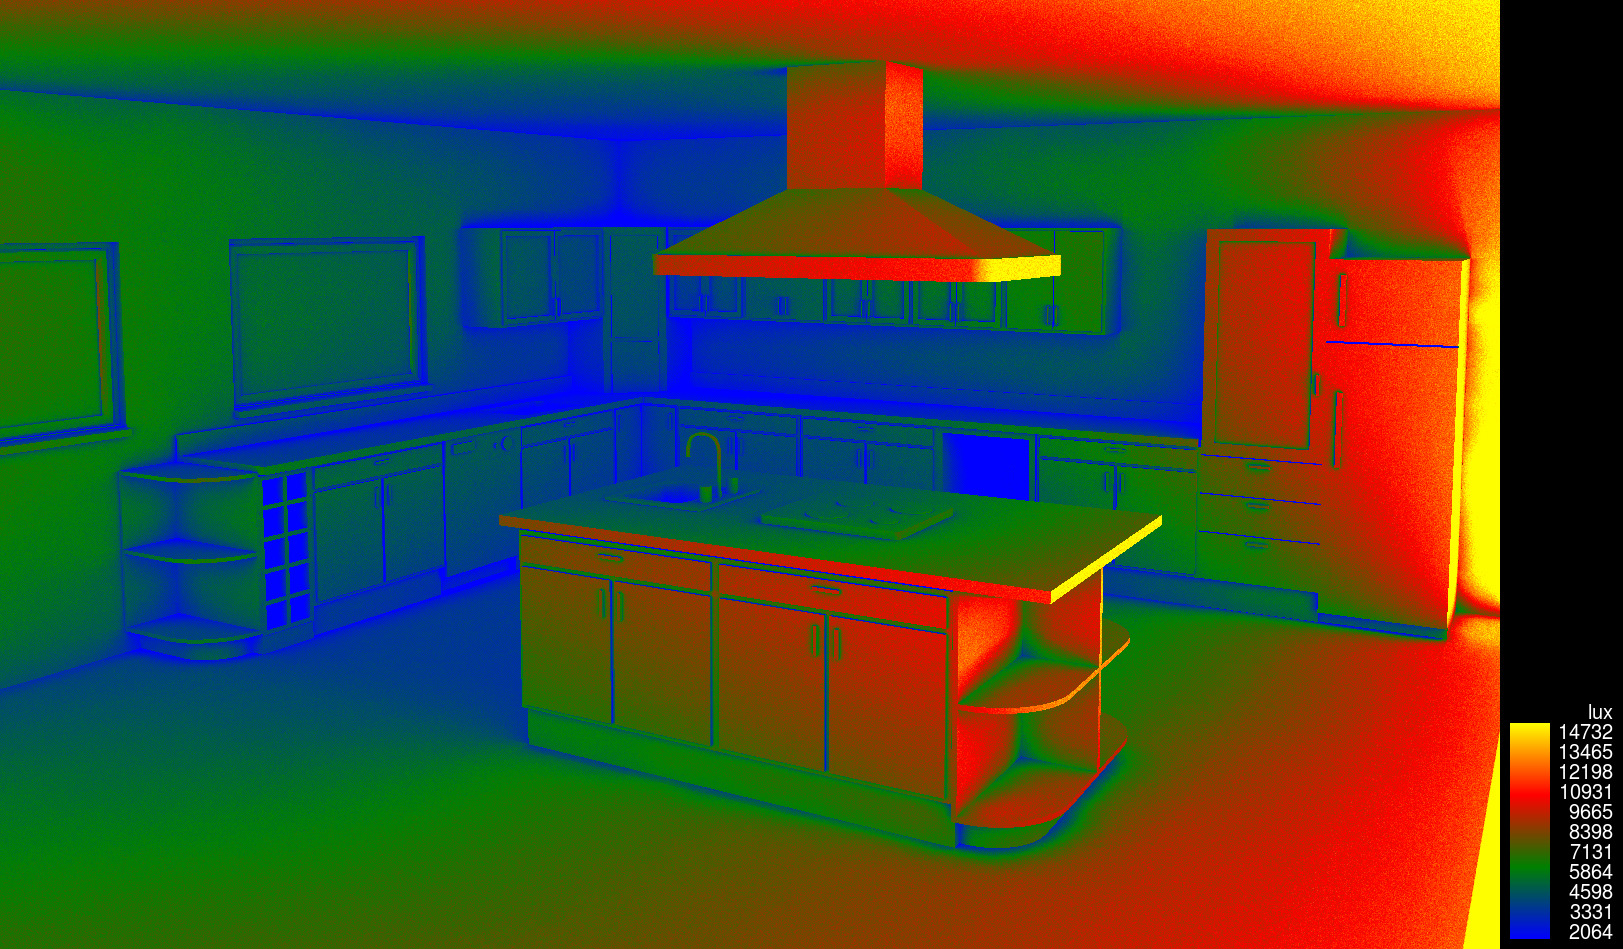
\includegraphics[width=1.00\textwidth]{img/KitchenIll.jpg}
	\caption{Illuminance Render of a Kitchen}
	\label{fig:KitchenIll}
\end{figure}


\end{document}